
\subsection{Binary Search Tree}
\begin{center}
 \deff{BST} или бинарное дерево поиска.
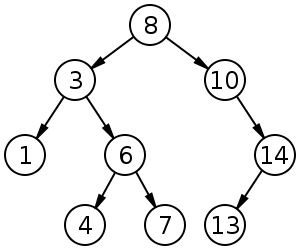
\includegraphics{assets/Binary_search_tree.png}    
\end{center}

Это абстрактный термин, существует множество разновидностей бинарных деревьев поиска, все они удовлетворяют нескольким аксиомам:
\begin{enumerate}
    \item Являются бинарными деревьями, что следует из названия(\href{https://ru.wikipedia.org/wiki/%D0%94%D0%B2%D0%BE%D0%B8%D1%87%D0%BD%D0%BE%D0%B5_%D0%B4%D0%B5%D1%80%D0%B5%D0%B2%D0%BE}{тык}, если вдруг не знаете, что это).
    \item В каждой вершины дерева записано значение, называемое его ключом.
    \item Если $v$ - вершина бинарного дерева со значением $x$, то все
    узлы в левом поддереве должны иметь ключи, меньшие $x$, а в правом поддереве
    большие $x$.
\end{enumerate}
%\deff{Полезный факт.} Если вам могут вставлять некоторые числа повторно, то вы можете у каждой вершины завести дополнительный параметр, равный числу данных элементов в структуре.
Список операций, доступных для дерева поиска:
\begin{enumerate}
    \item add(x)
    \item find(x)
    \item remove(x)
\end{enumerate}
Список операций у бинарных деревьев аналогичен списку операций у куч. 

\deff{Утверждение.} Все работает за $O(h)$, где $h$ - высота дерева.
\newpage
\deff{Доказательство:}
\begin{enumerate}
    \item add(x)
    
    Алгоритм:
    \begin{enumerate}
        \item Стартуем алгоритм с корня
        \item Если мы сейчас в вершине, сравниваем ключ, который в ней лежит и тот, что мы хотим добавить, в зависимости от этого идем в нужную сторону, чтобы выполнялось третье условие БДП.
        \item Если мы покинули дерево, то создаем новую вершину в том месте, где дерево было покинуто, она и будет вершиной с новым значением, заметим что ни одно из правил не нарушилось.
    \end{enumerate}
    \item find(x)
    
    Алгоритм:
    \begin{enumerate}
        \item Стартуем алгоритм с корня
        \item Если мы сейчас в вершине, сравниваем ключ, который в ней лежит и тот, что мы ищем, при равенстве мы победили и нашли искомый ключ, в противном случае идем в нужную сторону, пользуясь третьим условием БДП.
        \item Если мы покинули дерево, то искомого ключа в дереве нет.
    \end{enumerate}
    \item remove(x)
    
    Алгоритм:
    \begin{enumerate}
        \item Используем алгоритм поиска, который я описал выше и находим вершину, которую нужно удалить
        \item Тут есть несколько вариантов развития событий:
        \begin{enumerate}
            \item Если вершина не имеет потомков, то просто удаляем ее
            \item Если у вершины один потомок, то мы просто вырезаем ее, а потомка привязываем к родителю вершины.
            \item Если у вершины есть оба потомка, то попытаемся свести этот случай к предыдущему, для этого найдем вершину с одним потомком, которого мы можем поменять местами с нашей, так, чтобы свойства БДП не нарушились. Оказывается такая вершина существует, мы можем спуститься в правое поддерево и в нем постоянно идти влево, что приведет нас к наименьшей вершине, большей исходной. Теперь просто меняем их местами и вырезаем желаемую вершину.
            \begin{center}
                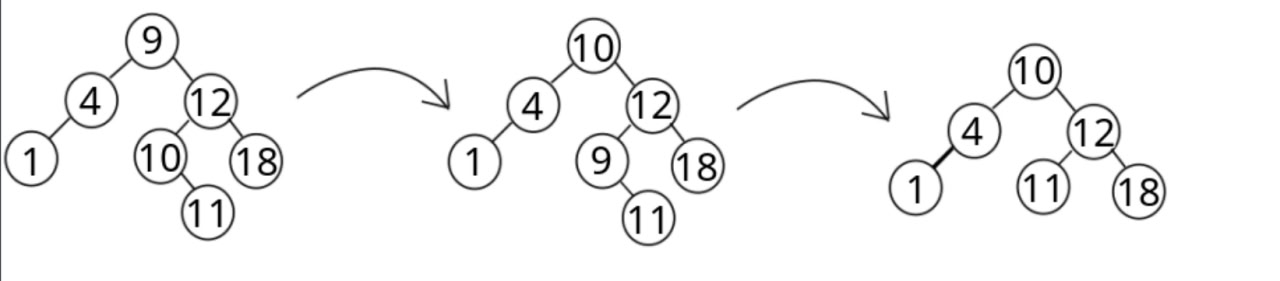
\includegraphics[width=15cm, height=3.5cm]{assets/example1.jpg}
            \end{center}
        \end{enumerate}
    \end{enumerate}
\end{enumerate}
\subsubsection{AVL-tree}
\deff{AVL-дерево} - бинарное дерево поиска, удовтлетворяющее свойству \textbf{сбалансированности}:
\begin{enumerate}
    \item [] Для каждой вершины модуль разницы высот у поддеревьев ее сыновей не превышает 1(если сын отсутствует, считаем глубину его поддерева равной 0). 
\end{enumerate}

Мы поддерживаем $h(x)$ --- количество вершин в поддереве, начинающегося с $x$.

$h(v) = max(h(L),h(R)) + 1 $.

\thmm{Лемма.} В дереве высоты $h$ хотя бы $F_h$ вершин ($h$ - ое число Фибоначчи)

\thmm{Доказательство:}
\begin{enumerate}
    \item []  Пусть $f(h)$ - min кол-во детей вершин в AVL c высотой $h$. Попытаемся вывести минимальное $f(h)$, через предыдущие. У нас обязательно есть 1 корень, у него потомок глубиной хотя бы $h-1$, и второй, глубиной хотя бы $h-2$ из-за сбалансированности дерева. Получаем формулу, которая крайне похожа на формулу чисел Фибоначчи:
    $$f(h) = f(h-1) + f(h-2) + 1$$
\end{enumerate}

Числа Фибоначчи растут экспоненциально, что означает, что глубина нашего дерева будет логарифмической, если мы сможем поддерживать сбалансированность, научимся же это делать.

\subsubsection{Балансировка AVL-tree}
Предположим мы теоритически научились балансировать поддеревья для данной вершины не ломая сбалансированность потомков, как пользоваться такой суперсилой? Давайте при изменении структуры дерева, начнем из вершины, в которой это изменение произошло, будем подниматься до корня и балансировать вершину, которую проходим. Эта идея позволит вернуть сбалансированность дереву, потому что глубины остальных поддеревьев при добавлении/удалении не поменялись, а в тех вершинах, где что-то могло сломаться, мы все починили.

Ну а балансировать поддеревья сыновей фиксированной вершины нам поможет данный агрегат:
\begin{center}
   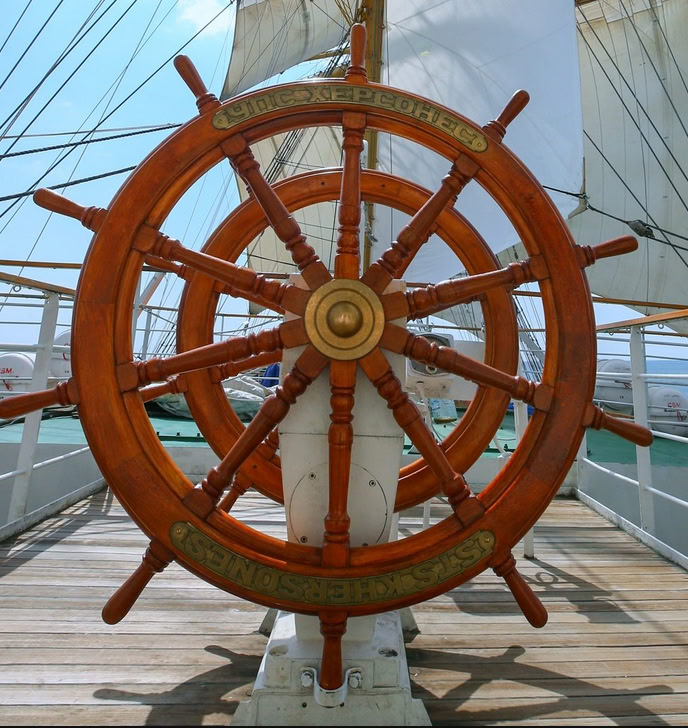
\includegraphics[width=8cm, height=8cm]{assets/wheel.jpg}
\end{center}

Всего существует 4 типа поворотов, я подскажу вам как их проще всего запомнить, если вы хотите сделать глубже поддерево правого сына, то вам нужно перекинуть туда вершины с левого поддерева, то есть повернуть штурвал вправо - поворот правый, иначе влево - поворот левый. Но это только первый критерий, есть еще второй - размер вращения. Если вам надо переместить всего 2 вершины и поддеревья, то это вращение малое, если же 3 вершины и поддеревья, то большое.

Я буду показывать только правые повороты, так как левые просто симметричны. Вот схема малого поворота:
\begin{center}
    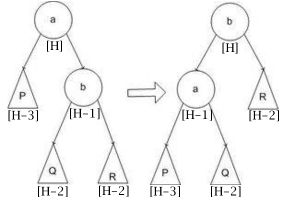
\includegraphics[width=8cm, height=5cm]{assets/avl_balance1.jpg}
\end{center}
Он подойдет вам если глубина поддерева $R$ равна $h-2$. При том, даже если глубина $Q$ будет $h-3$, все равно балансированность дерева не нарушиться. Проверку этого замечательного факта и схемы я оставлю читателю, тут нечего особо обсуждать.
 
В том случае, если глубина $R$ внезапно оказалась равна $h-3$, нам придется использовать большой правый поворот:
\begin{center}
    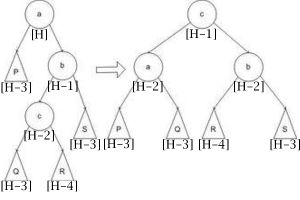
\includegraphics[width=10cm, height=7cm]{assets/avl_balance2.jpg}
\end{center}

Тут на самом деле надо поразбирать вариантики, чему могут быть равный глубины поддеревьев $Q$ и $R$, но проще заметить, что $P$ и $S$ всегда $h-3$, а мощности $Q$ и $R$ либо $h-3$, либо $h-4$, из чего уже становится понятно, что у полученных в результате поворота поддеревьев вершин $a$ и $b$ глубины действительно равны $h-2$. Ну а задание убедиться в том, что остальные свойства БДП выполняются при таком повороте я опять же оставлю читателю.

Последнее, что я хочу тут записать - как запомнить сами схемы поворота, попробуйте запомнить только перемещение вершин относительно друг друга, а перемещение поддеревьев восстановите автоматически. 